\chapter{Background}


\section{Past Solution}

In the NASA space challenge website, many participants had offered their solution by machine learning or did their prediction by the flight timetable and route. However, these methods usually only can be used to find the existence of contrails, or the possibility of those contrails exist. Meanwhile, it really relies on the flight data and the photo location, but it is not convenient for scientists to access all the flight database.\\

Here are some examples:
\begin{itemize}
\item \href{https://2016.spaceappschallenge.org/challenges/aero/clouds-or-contrails/projects/contrailers-exeter}{Contrailers-Exeter} \\
The team mentioned in their explanation that they determine the probability of contrails by examining recent flights in the area and the air temperature. 
\item \href{https://2016.spaceappschallenge.org/challenges/aero/clouds-or-contrails/projects/hot-on-the-contrail}{Hot on the Contrail}\\
They do a machine learning solution, however, they only determine the possibility of contrails existing, but not where contrails are. This solution has been done the NASA space challenge, but it seems not useful for detecting the actual contrails locations.  
\end{itemize}

\section{Aim and Target}

In order for scientists to do better researchers on contrails and clouds, the aim of this project proposes a program to automatically segment the contrails from clouds on different kinds of images, such as satellites images, photos, and so on. After the contrails in the image have been determined, they are highlighted and a comparison image is outputted.

\newpage
\section{Scope and Constraints}
\begin{itemize}
    \item This project will not be able to use the images with interference information, such as “figure1.jpg” (figure below) which has latitude and longitude lines and map boards. Those lines have much clearer border than the clouds image, and they will disrupt the detection result.
    \begin{figure}[htb]
        \centering
        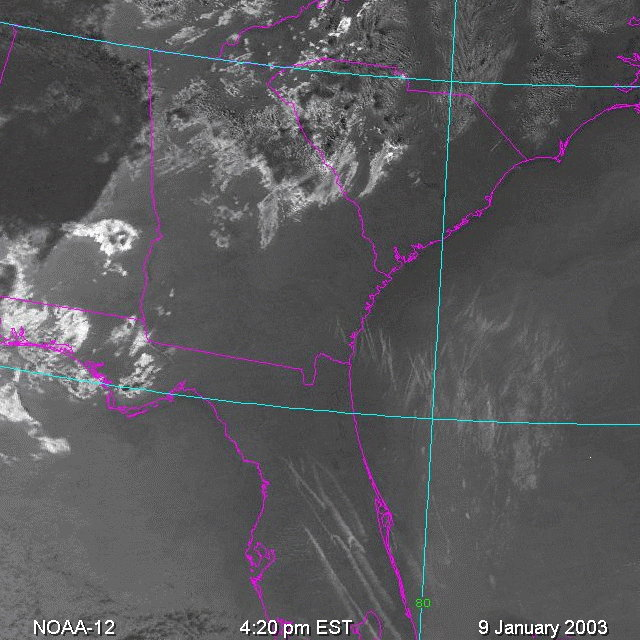
\includegraphics[scale=0.5]{pic/figure1.jpg}
        \caption[Short form for the mapping directory]{"figure1.jpg"}
    \end{figure}
    \item Our program may be inefficient to process large images. The strategical removal of non-line edgels is complicatedly expensive.
\end{itemize}